\section{Overview}

\subsection{Architectural style}
\mbox{}\newline
 We decided to use the MVC pattern as the basic architectural style for the Calendar system.
\newline
\newline
The MVC pattern separates data and user interface and has Controller as a intermediated component. The pattern is used when there are multiple ways to view and interact with data.
\newline
\newline
MVC is a abbreviation for Model View Controller. The software is divided in these components. The components are defined as following:
\begin{itemize}
	\item \textbf{Model} handles data.
	\item \textbf{View} is attached to model and presents the data.
	\item \textbf{Controller} is the link between model and view. 
\end{itemize}
\bigskip


To get an overview of the MVC pattern we outlined the pros and cons.
\newline
\textbf{Pros}
\begin{itemize}
	\item low coupling
	\item high cohesion
	\item code maintenance
	\item code reuse
\end{itemize}
\textbf{Cons}
\begin{itemize}
	\item code complexity
	\item development time
\end{itemize}

\newpage
In our Object Oriented Analysis an Analysis Object Model was defined where we identified:
\begin{itemize}
	\item Entity objects (\emph{model})
	\item Boundary objebts (\emph{view})
	\item Control objects (\emph{controller})
\end{itemize}

The Analysis Object Model is a simplification of MVC pattern. It made it eaiser to set up the MVC pattern and build further on the Object Oriented Design. 

\subsection{UML Class diagram}
Our main program is in the MVC pattern.The Model is used to keep the information about \textit{Calendar}, \textit{Events}, \textit{Client} and \textit{Alarms}. The \textit{Controller} deals with modification of the model, e.g. synchronize and share events. The view consist of our main view and our forms, these forms are used by the client to input information that the controller then saves in the model or database.
When we want to synchronize our \textit{Calendar} we need to connect to the database, through our \textit{SyncSubsystem}, here is where the strategy pattern comes in. The strategy pattern observes whether we have a connection to the internet or not. Then the information will be sent on to the bridge pattern. By now we know which kind of storage we would like to use. When the right one is selected the storage will be built by our factory pattern. 
Furthermore we have implemented the adapter pattern as an extension of our \textit{SyncSubsystem}, this has an outgoing connection from google calendar. The information that the google calendar wants to extract will then be sent to the \textit{ICalendarEntry} and further on to the right adapter that will handle the transformation to our system. 
We have also implemented Composite pattern but it is a very weak implementation because we do not think that it has any relevance in our program. We already had the repeat event implemented in our own system. The Composite pattern has a connection to the events in our model. The Composite pattern is used for repeating events.
\newline
The UML Class diagram shows our three subsystems and the connections between them. Whenever a user likes to synchronize his calendar, a connection from \textit{UpdateControl} in the \textit{CalendarManagementSubsystem} will set to \textit{NetworkConnection} in our \textit{SyncSubsystem}.
The connection between our \textit{SyncSubsystem} and our \textit{CalendarManagementSubsystem} is between the interface \textit{IShare} and \textit{NotifyUserControl}. Which is the controller that sends the invite out, and then the interface will handle it at the other end. Here is space for different share systems e.g. \textit{Facebook}. 
\newline
\newline
The \textit{UML Class diagram} is on next page.

\begin{sidewaysfigure}
\centering
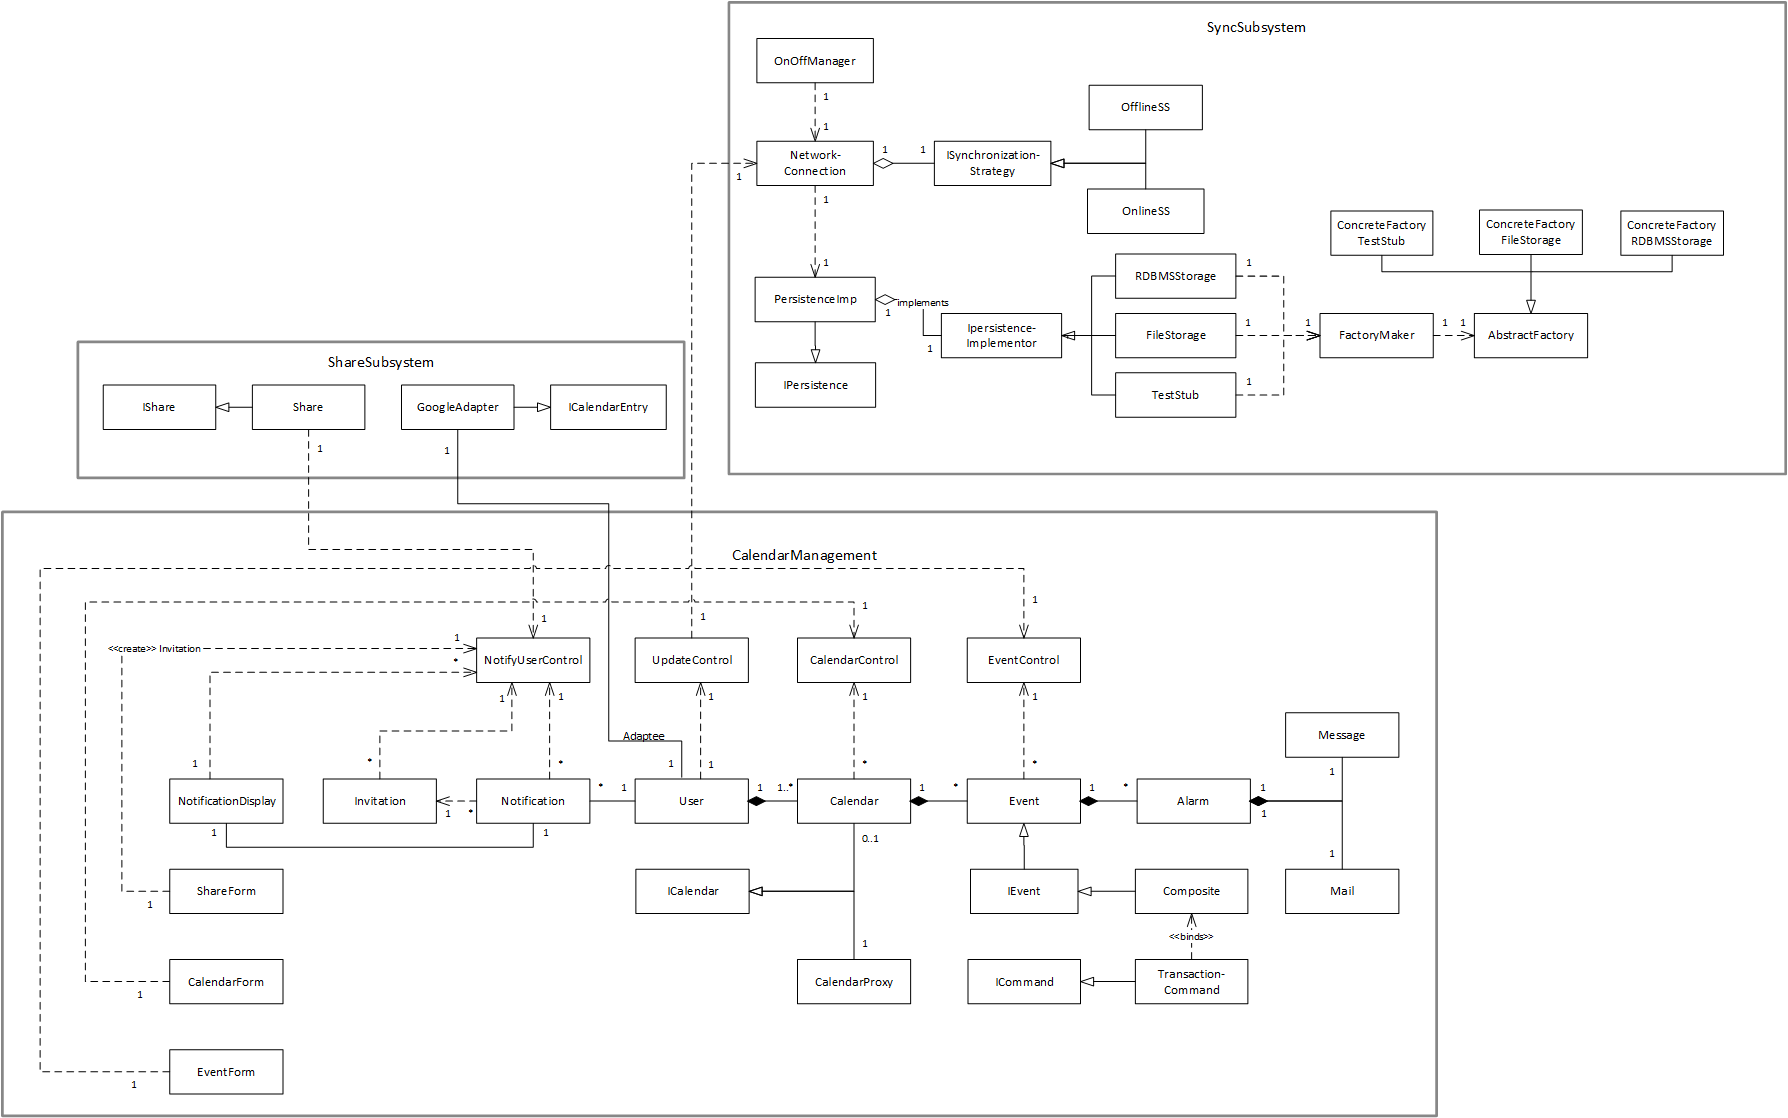
\includegraphics[width=210mm]{UMLClassDiagram.png}
\caption{UML Class diagram \label{img:UMLClassDiagram}}
\end{sidewaysfigure}
